\documentclass[11pt, addpoints, answers]{exam}

\usepackage[utf8]{inputenc}
\usepackage[T1]{fontenc}
\usepackage[margin  = 1in]{geometry}
\usepackage{amsmath, amscd, amssymb, amsthm, verbatim}
\usepackage{mathabx}
\usepackage{setspace}
\usepackage{float}
\usepackage{color}
\usepackage{graphicx}   
\usepackage[colorlinks=true]{hyperref}
\usepackage{tikz}

\usetikzlibrary{shapes,arrows}
%%%<
\usepackage{verbatim}
%%%>
\usetikzlibrary{automata,arrows,positioning,calc}

\usetikzlibrary{trees}

\shadedsolutions
\definecolor{SolutionColor}{RGB}{214,240,234}

\newcommand{\bbC}{{\mathbb C}}
\newcommand{\R}{\mathbb{R}}            % real numbers
\newcommand{\bbR}{{\mathbb R}}
\newcommand{\Z}{\mathbb{Z}}            % integers
\newcommand{\bbZ}{{\mathbb Z}}
\newcommand{\bx}{\mathbf x}            % boldface x
\newcommand{\by}{\mathbf y}            % boldface y
\newcommand{\bz}{\mathbf z}            % boldface z
\newcommand{\bn}{\mathbf n}            % boldface n
\newcommand{\br}{\mathbf r}            % boldface r
\newcommand{\bc}{\mathbf c}            % boldface c
\newcommand{\be}{\mathbf e}            % boldface e
\newcommand{\bE}{\mathbb E}            % blackboard E
\newcommand{\bP}{\mathbb P}            % blackboard P

\newcommand{\ve}{\varepsilon}          % varepsilon
\newcommand{\avg}[1]{\left< #1 \right>} % for average
%\renewcommand{\vec}[1]{\mathbf{#1}} % bold vectors
\newcommand{\grad}{\nabla }
\newcommand{\lb}{\langle }
\newcommand{\rb}{\rangle }

\def\Bin{\operatorname{Bin}}
\def\Var{\operatorname{Var}}
\def\Geom{\operatorname{Geom}}
\def\Pois{\operatorname{Pois}}
\def\Exp{\operatorname{Exp}}
\def\Weibull{\operatorname{Weibull}}
\newcommand{\Ber}{\operatorname{Ber}}
\def\Unif{\operatorname{Unif}}
\def\No{\operatorname{N}}
\newcommand{\E}{\mathbb E}            % blackboard E
\def\th{\theta }            % theta shortcut
\def\V{\operatorname{Var}}
\def\Var{\operatorname{Var}}
\def\Cov{\operatorname{Cov}}
\def\Corr{\operatorname{Corr}}
\newcommand{\epsi}{\varepsilon}            % epsilon shortcut

\providecommand{\norm}[1]{\left\lVert#1\right\rVert} %norm
\providecommand{\abs}[1]{\left \lvert#1\right \rvert} %absolute value

\DeclareMathOperator{\lcm}{lcm}
\newcommand{\ds}{\displaystyle}	% displaystyle shortcut

% Distributions.
% \newcommand*{\UnifDist}{\mathsf{Unif}}
% \newcommand*{\ExpDist}{\mathsf{Exp}}
% \newcommand*{\DepExpDist}{\mathsf{DepExp}}
% \newcommand*{\GammaDist}{\mathsf{Gamma}}
% \newcommand*{\LognormalDist}{\mathsf{LogNorm}}
% \newcommand*{\WeibullDist}{\mathsf{Weib}}
% \newcommand*{\ParetoDist}{\mathsf{Par}}
% \newcommand*{\NormalDist}{\mathsf{Normal}}

% \newcommand*{\GeometricDist}{\mathsf{Geom}}
% \newcommand*{\NegBinomialDist}{\mathsf{NegBin}}
% \newcommand*{\BinomialDist}{\mathsf{Bin}}
% \newcommand*{\PoissonDist}{\mathsf{Poisson}}
\newcommand*{\Prob}{\mathbb{P}}
% \newcommand*{\Cov}{\mathsf{Cov}}


\def\semester{2022-2023}
\def\course{Modèle de Durée}
\def\title{\MakeUppercase{Examen final}}
\def\name{Pierre-O Goffard}
%\def\name{Professor Wildman}

\setlength\parindent{0pt}

\cellwidth{.35in} %sets the minimum width of the blank cells to length
\gradetablestretch{2.5}

%\bracketedpoints
%\pointsinmargin
%\pointsinrightmargin

\begin{document}


\runningheader{\course  \vspace*{.25in}}{}{\title \vspace*{.25in}}
%\runningheadrule
\runningfooter{}{Page \thepage\ of \numpages}{}

% \firstpageheader{Name:\enspace\hbox to 2.5in{\hrulefill}\\  \vspace*{2em} Section: (circle one) TR: 3-3:50 \textbar\, TR: 5-5:50 \textbar\,  TR: 6-6:50(Xu) \textbar\,  TR: 6-6:50 }{}{Perm \#: \enspace\hbox to 1.5in{\hrulefill}\\ \vspace*{2em} Score:\enspace\hbox to .6in{\hrulefill} $/$\numpoints}
\extraheadheight{.25in}

\hrulefill

\vspace*{1em}

% Heading
{\center \textsc{\Large\title}\\
	\vspace*{1em}
	\course -- \semester\\
	Pierre-O Goffard\\
}
\vspace*{1em}

\hrulefill

\vspace*{2em}

\noindent {\bf\em Instructions:} On éteint et on range son téléphone.
\begin{itemize}
	\item La calculatrice et les appareils éléctroniques ne sont pas autorisés.
	\item Vous devez justifier vos réponses de manière claire et concise.
	\item Vous devez écrire de la manière la plus lisible possible. Souligner ou encadrer votre réponse finale.
	\item \underline{Document autorisé:} Une feuille manuscrite recto-verso

\end{itemize}


\begin{center}
	\gradetable[h]
\end{center}

\smallskip

\begin{questions}
\question Soient deux variables aléatoires $E\sim \Exp(\lambda)$ et $W\sim\Weibull(\alpha, \beta)$, mutuellement indépendantes, de densité respective
$$
f_E(x)  = \lambda e^{-\lambda x}\text{, et }f_W(x)  = \frac{\alpha}{\beta}\left(\frac{x}{\beta}\right)^{\alpha-1}e^{-(x/\beta)^\alpha},
$$
pour $x>0$. On définit également $T = \min(E, W)$, il s'agit d'un modèle de risques concurrents.
\begin{parts}
\part[2] Rappeler la définition de la fonction de hasard, et donner l'expression des fonctions de hasard de $E$ et $W$.
\begin{solution}
La fonction de hasard est défini par 
$$
h(x) = \frac{f(x)}{S(x)},
$$
où $f$ et $S$ sont la densité et la fonction de survie respectivement. Pour les deux modèle considéré on a 
$$
h_E(x) = \lambda,\text{ et }h_W(x) = \frac{\alpha}{\beta}\left(\frac{x}{\beta}\right)^{\alpha-1}.
$$
\end{solution}
\part[1] Calculer $S(t)=\Prob(T>t)$, la fonction de survie de $T$. 
\begin{solution}
$$
S(t) = \Prob(T>t)=\Prob(\min(E, W)>t)=S_E(t)S_W(t)=\exp(-\lambda x - (x/\beta)^\alpha)
$$
\end{solution}
\part[1] Calculer $h(t)$ la fonction de hasard de $T$.
\begin{solution}
On a 
$$
f(t) = S'(t) = f_E(t)S_W(t) + S_E(t)f_W(t).
$$
On en déduit que 
$$
h(t) = h_E(t)+h_W(t)= \lambda + \frac{\alpha}{\beta}\left(\frac{t}{\beta}\right)^{\alpha-1}
$$
\end{solution}
\part[1] Nous disposons d'un jeu de $n$ observations iid, notées $t_1,\ldots, t_n$, de $T$ censurées à droite. Donner l'expression de la vraisemblance du modèle pour ces données censurées. Vous devez rappeler les notations utilisées habituellement.
\begin{solution}
Soient $t_1,\ldots, t_n$, les données disponibles sont données par
$$
\mathcal{D} = (x_i,\delta_i) = (t_i\land c_i,\mathbb{I}_{t_i\leq c_i})
$$
où $c_1,\ldots, c_n$ sont les réalisations de la variable de censure. La vraisemblance s'écrit
$$
\mathcal{L}(\mathcal{D},\theta) = \prod_{i=1}^n h(x_k)^{\delta_i}S(x_k),
$$
où $\theta = (\lambda, \alpha, \beta)$.
\end{solution}
\end{parts}
\question Le tableau \ref{tab:mortality_data_NLD} est un extrait d'un jeu de données comprenant les expositions initiales et nombre de décès  dans la population Néerlandaise pour l'année $2000$.
\begin{table}[ht!]
\centering
\begin{tabular}{lll}
  \hline
 Age & $E_x^0$&$D_x$ \\ 
  \hline
 0 & 204,776 & 1,059 \\ 
  1 & 202,369 & 94 \\ 
  2 & 196,887 & 59 \\ 
 $\vdots$ &$\vdots $\\
  108 & 3 & 2 \\ 
  109 & 1 & 0 \\ 
  110+ & 3 & 0 \\ 
   \hline
\end{tabular}
\caption{Extrait des données de mortalités au Pays-Bas.}
\label{tab:mortality_data_NLD}
\end{table}
\begin{parts}
\part[2] Donner l'expression des probabilités de décès à l'âge $x$ notées $\widehat{q}_x$ en fonction de $E_x^0$. Rappeler les hypothèses du modèle sous jacent et à quoi correspond $E_x^0$. 
\begin{solution}
$E_x^0$ est l'exposition initiale. On utilise le modèle binomial suivant lequel le nombre de décès à l'âge $x$ suit une loi binomiale
$$
D_x\sim\Bin(E_x^0,q_x).
$$
Dans le cadre de ce modèle, on estime la probabilité de décès par 
$$
\widehat{q}_x=\frac{D_x}{E_{x}^0}.
$$
\end{solution}

% \part[1] 

\part[2] Les probabilités de décès "brutes" sont données sur la Figure \ref{fig:taux_brut}. A quoi correspondent les lignes pointillés sur la Figure \ref{fig:taux_brut}? Comment les obtient-on?
\begin{solution}
Les lignes pointillées forment un intervalle de confiance autour des taux bruts. On sait que 
$$
\widehat{q_x}\sim\No\left(q_x,\frac{q_x(1-q_x)}{E^0_x}\right).
$$
On en déduit que l'intervalle de confiance de niveau $\alpha$ est donnée par 
$$
q_x\in\left[\widehat{q_x} - z_{\alpha/2}\sqrt{\frac{q_x(1-q_x)}{E^0_x}}, \widehat{q_x} + z_{\alpha/2}\sqrt{\frac{q_x(1-q_x)}{E^0_x}}\right].
$$
\end{solution}
\begin{figure}[h]
\centering
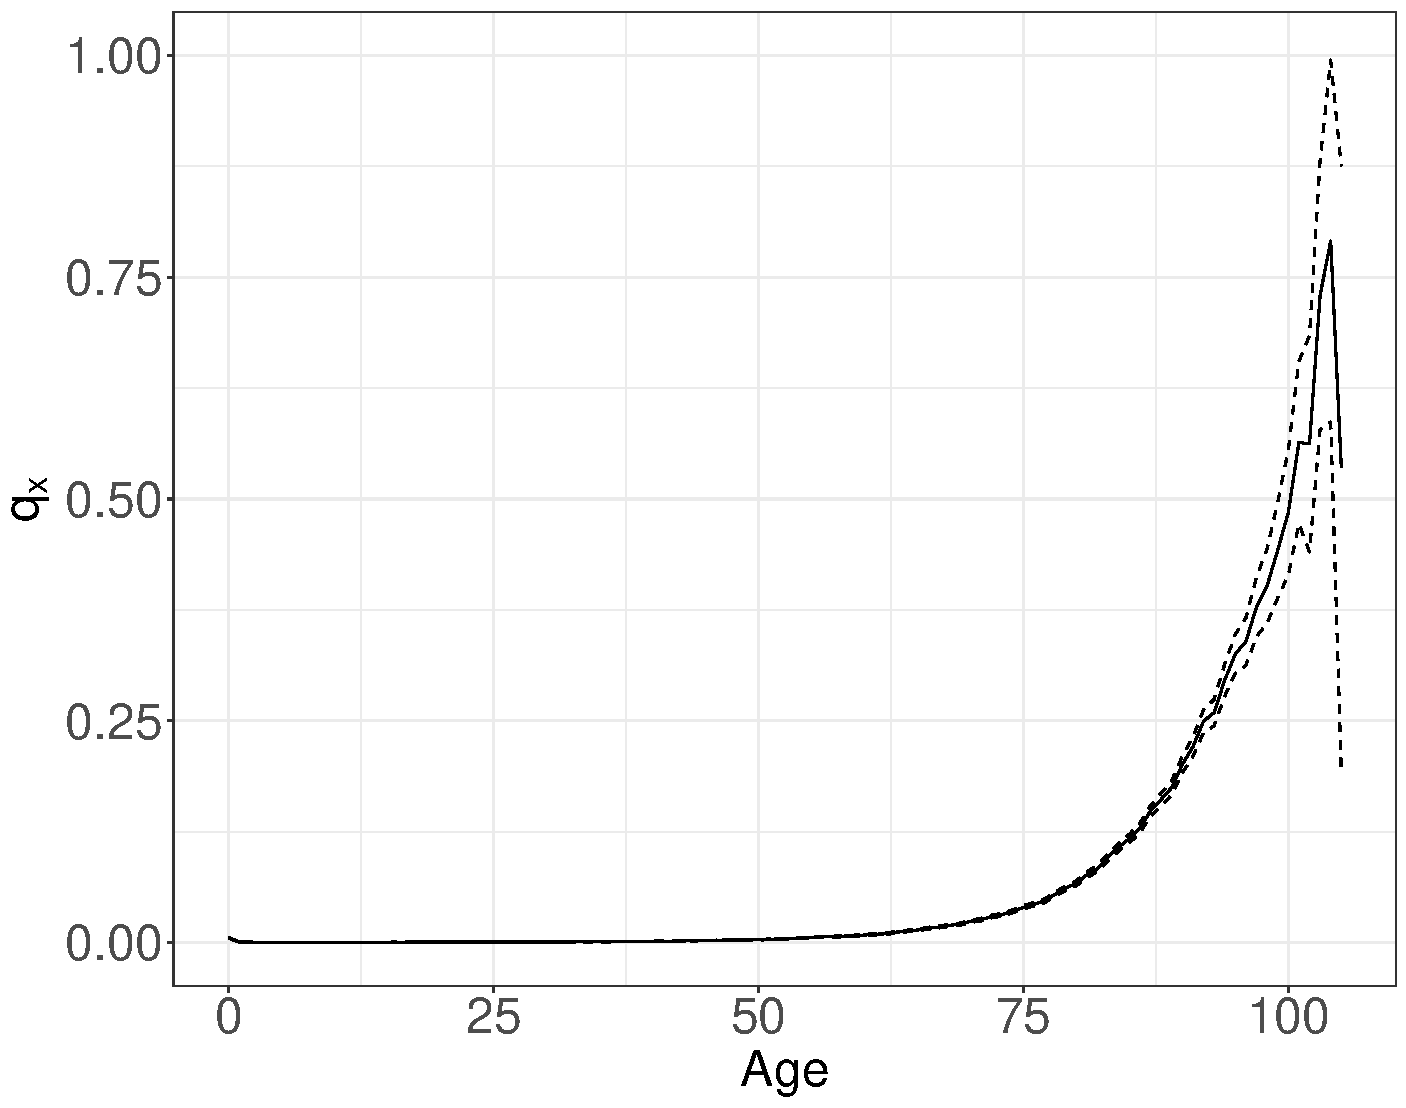
\includegraphics[width = 0.6\textwidth]{taux_brut}
\caption{Probabilités de décès brutes}
\label{fig:taux_brut}
\end{figure}
\part[2] Quels sont les deux traitements à appliquer sur ces probabilités de décès pour obtenir une estimation finale des probabilité de décès jusqu'à l'âge $115$? Vous devez détailler une méthode pour réaliser chacun des deux traitements.
\begin{solution}
Il faut appliquer une méthode de lissage etune méthode de fermeture de table. Les méthodes sont décrites dans le cours.
\end{solution}
\part[1] Donner une formule d'estimation de la fonction de survie $\widehat{S}(x)$ de $X$, la variable aléatoire égale à l'âge de décès. On donnera cette formule en fonction des $\widehat{q}_x$.
\begin{solution}
On peut estimer la fonction de survie par 
$$
\widehat{S}(x)=\prod_{k=0}^{x-1}(1-\widehat{q}_k)\text{, pour } x>1,
$$
et $S(0)=1$.
qui correspond à l'estimateur de Kaplan-Meier.
\end{solution}
\part[1] Un extrait de la table de mortalité issue des taux bruts est donné dans le Tableau \ref{tab:mortality_table_NLD}.
\begin{table}[ht!]
\centering
\begin{tabular}{ll}
  \hline
 Age & $l_x$ \\ 
  \hline
 0 & 100,000 \\ 
  1 & 99,482 \\ 
  2 & 99,436 \\ 

 $\vdots$ &$\vdots $\\
  104 & 9 \\ 
  105 & 1 \\ 
  106 & 0 \\ 
   \hline
\end{tabular}
\caption{Extrait de la table de mortalités au Pays-Bas pour l'année $2000$.}
\label{tab:mortality_table_NLD}
\end{table}
Comment est obtenue cette table ? A quoi correspond $l_x$?
\begin{solution}
On décide d'un radix, ici $l_0=100,000$ puis
$$
l_x= l_0\cdot \widehat{S}(x),\forall x.
$$
\end{solution}

\part[1] Le modèle de Gompertz-Makeham suppose que la variable aléatoire $X$ admet une fonction de hasard de la forme
$$
h(x) = a+bc^x,\text{ }x\in \mathbb{R}_+.
$$
Soit $\theta = (a,b,c)$. Montrer que les probabilités de décès s'écrivent sous la forme 
$$
q_x(\theta) = 1- sg^{c^x(c-1)},
$$
où vous exprimerez $s$ et $g$ en fonction de $a,b$ et $c$
\begin{solution}
On a 
\begin{eqnarray*}
q_x(\theta) &=& 1-\exp\left(-\int_{x}^{x+1}a+bc^x\text{d}x\right)\\
&=& 1-\exp\left(-a-b\int_{x}^{x+1}e^{x\log(c)}\text{d}x\right)\\
&=& 1-e^a\exp\left(-\frac{b}{\log(c)}c^x(c-1)\right)\\
\end{eqnarray*}
On en déduit que 
$$
q_x(\theta) = 1- sg^{c^x(c-1)},
$$
avec $s=e^{-a}$ et $g = e^{-b/\log(c)}$.
\end{solution}
\part[1] Montrer que pour $q_x(\theta)$ proche de $0$, on a 
$$
q_x(\theta)\approx -\log(s) - \log(g)(c-1)c^x.
$$
\underline{Indication}: On pourra utiliser un développement limité.
\begin{solution}
Pour $q_x(\theta)$ proche de $0$, on a 
$$
q_x(\theta)\approx-\log(1-q_x(\theta)) = -\log(s) - \log(g)(c-1)c^x.
$$ 
\end{solution}
\part[2] En utilisant la question précédente identifier les coefficients $\alpha$ et $\beta$ tel que
$$
\log(q_{x+1}(\theta)-q_{x}(\theta))\approx \alpha +\beta x
$$
en fonction de $\theta$. En déduire une méthode d'estimation pour $g$ et $c$.
\begin{solution}
En utilisant l'approximation de la question précédente, il vient 
\begin{eqnarray*}
\log(q_{x+1}-q_{x})&\approx& \log\left[ \log(1/g)(c-1)^2c^x\right]\\
&=&\log(\log(1/g))+2\log(c-1) + x\log(c)\\
&=&\alpha +\beta x
\end{eqnarray*}
Cette relation suggère une regression linéaire de $\log(q_{x+1}-q_{x})$ sur $x$ et donc une estimation de $\alpha$ et $\beta$ par les moindre carrés ordinaires.
\end{solution}
\part[1] En supposant connu $g$ et $c$, comment estimer $s$?
\begin{solution}
On reprend l'aproximation précédente
$$
q_x(\theta)\approx -\log(s) - \log(g)(c-1)c^x.
$$
On peut donc écrire 
$$
s= \exp(-q_x - c^x(c-1)\log(g))
$$
et prendre la moyenne pour tout $x$ par exemple.
\end{solution}
\part[1] La Figure \ref{fig:taux_smooth_makeham} montre les probabilités de décès issues de la table de mortalité \ref{tab:mortality_data_NLD} et du modèle de Makeham. Quels commentaires peut-on faire?
\begin{solution}
L'ajustement aux taux lissés n'est pas parfait. On constate une sur-estimation de la mortalité aux jeunes âges et une sous-estimation aux âges élevés.
\end{solution}
\begin{figure}[h]
\centering
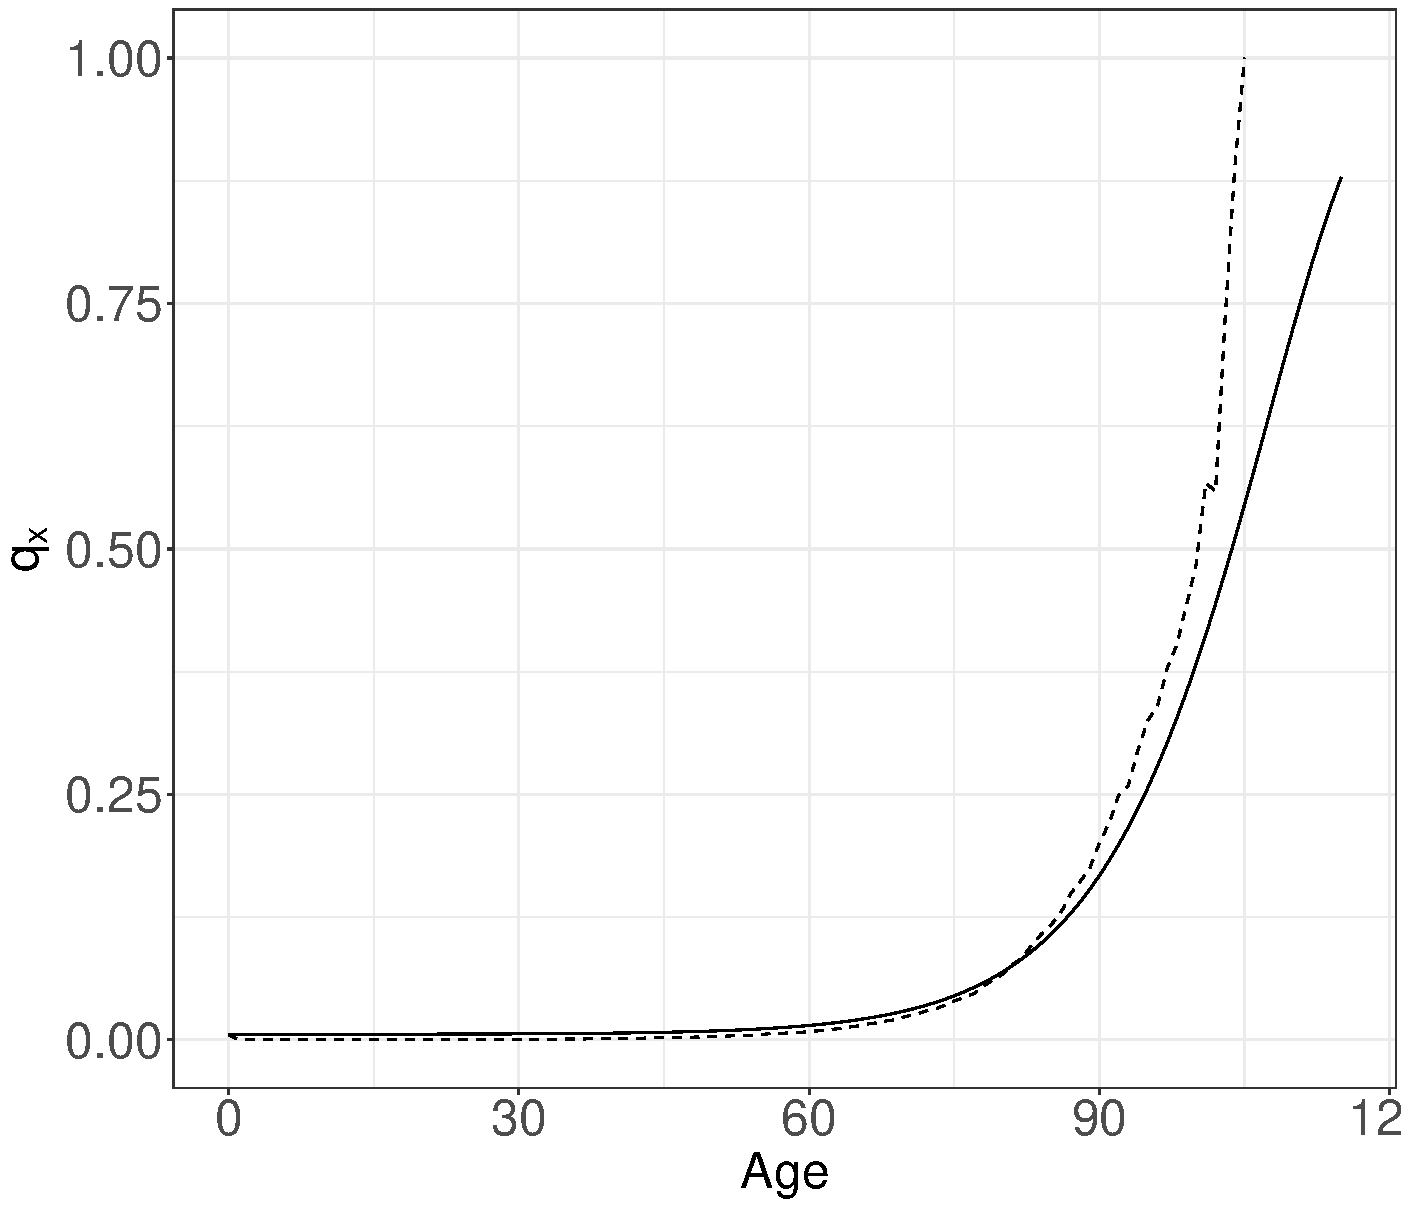
\includegraphics[width = 0.6\textwidth]{taux_smooth_makeham}
\caption{Probabilités de décès issues de la table de mortalité \ref{tab:mortality_table_NLD} (pointillé) et du modèle de Makeham (trait plein).}
\label{fig:taux_smooth_makeham}
\end{figure}
\part[1] La Figure \ref{fig:reg_plots} montre les graphiques de $\log(q_{x+1}-q_x)$ et $\exp(-q_x - c^x(c-1)\log(g))$ en fonction de $x$.
\begin{figure}[h]
\centering
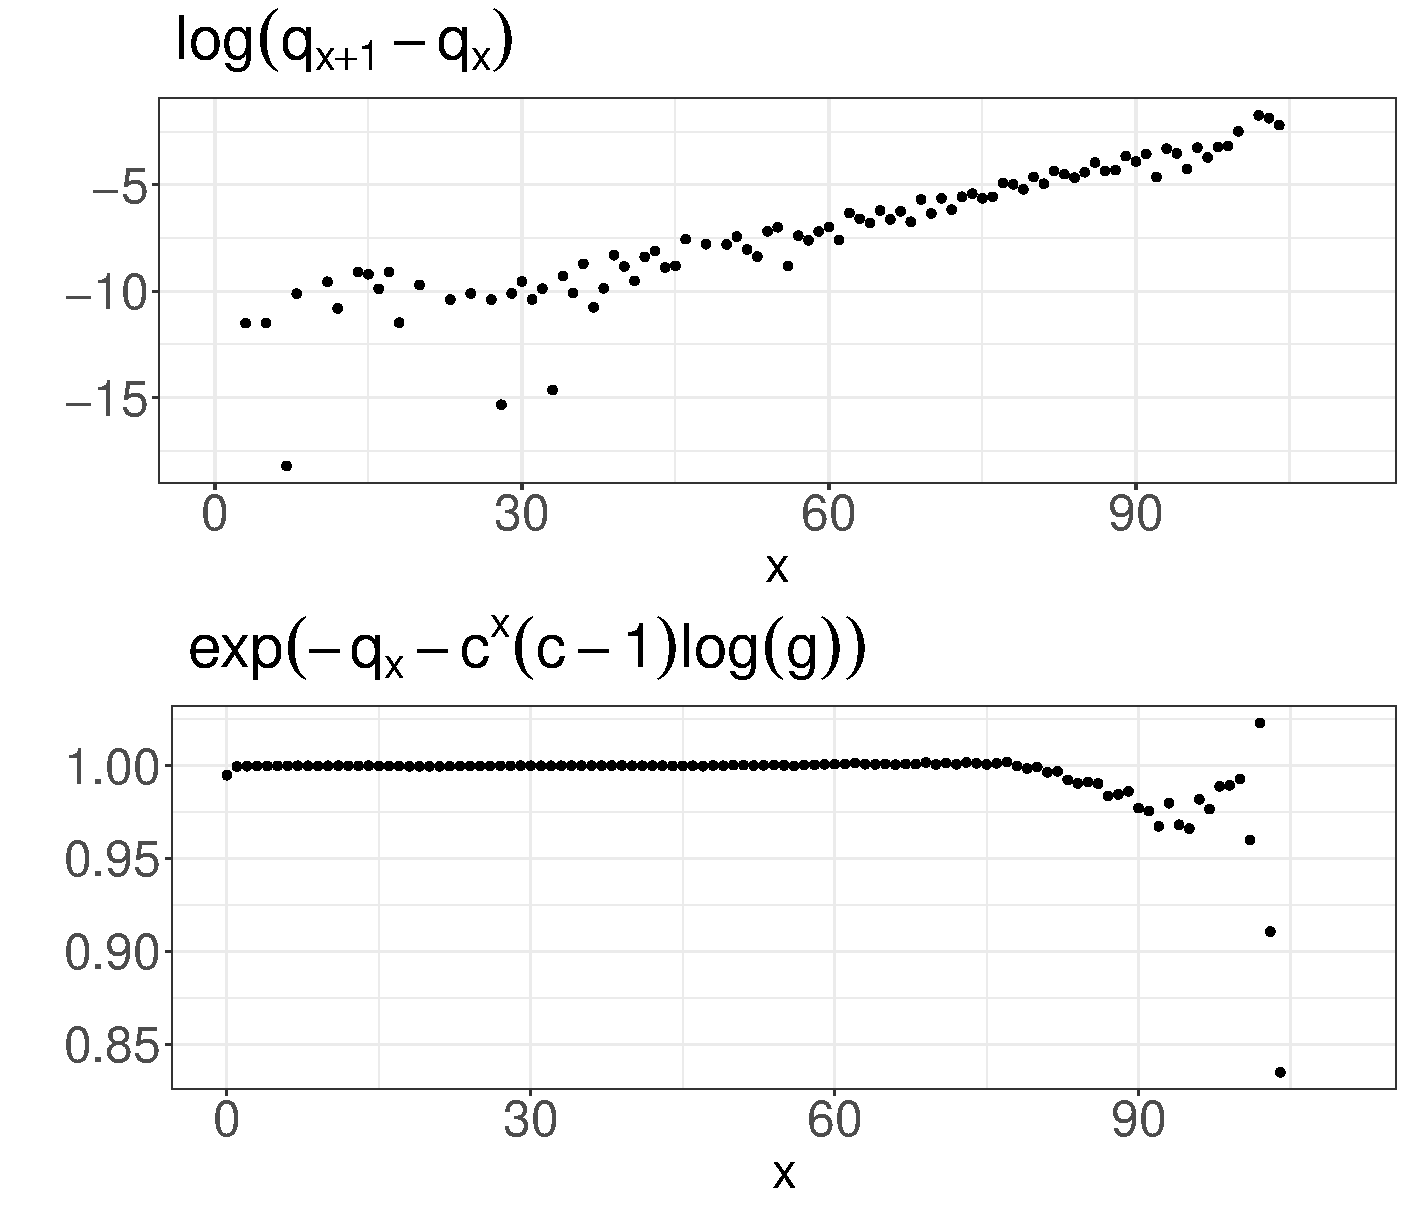
\includegraphics[width = 0.7\textwidth]{reg_plots}
\caption{$\log(q_{x+1}-q_x)$ et $\exp(-q_x - c^x(c-1)\log(g))$ en fonction de $x$.}
\label{fig:reg_plots}
\end{figure}
Comment pourrait-on améliorer l'ajustement du modèle de Makeham de la Figure \ref{fig:taux_smooth_makeham}?
\begin{solution}
Une solution serait d'introduire une pondération $(w_x)$ des âges $x$, en supprimant par exemple les valeurs aberrantes visibles sur la figure \ref{fig:reg_plots}.
\end{solution}
\end{parts}
 \end{questions}
%  \clearpage
% %-------------------------------TABLE-------------------------------
% \newpage
% \hrule
% \vspace*{.15in}
% \begin{center}
%   \large\MakeUppercase{Formulaire}
% \end{center}
% \vspace*{.15in}
% \hrule
% \vspace*{.25in}

% \renewcommand\arraystretch{3.5}
% \begin{table}[H]
% \begin{center}
% \footnotesize
% \begin{tabular}{|c|c|c|c|c|c|}

% \hline
% Nom & abbrev. & Loi & $\E(X)$ & $\Var(X)$ & FGM\\
% \hline\hline
% Binomial & $\Bin(n,p)$ & $\binom{n}{k}p^k(1-p)^{n-k}$ & $np$ & $np(1-p)$ & $[(1-p)+pe^t]^n$\\
% \hline
% Poisson & $\Pois(\lambda)$ & $e^{-\lambda}\dfrac{\lambda^k}{k!}$ & $\lambda$ & $\lambda$ &$ \exp(\lambda(e^t-1))$\\
% \hline
% Geometric & $\Geom(p)$ & $(1-p)^{k-1}p$ & $\dfrac{1}{p}$ & $\dfrac{1-p}{p^2}$ & $\frac{pe^t}{1-(1-p)e^t}$ pour  $t<-\ln(1-p)$\\
% \hline
% Uniform & $\Unif(a,b)$ & $\begin{cases} \dfrac{1}{b-a} & a\leq t\leq b\\ 0 & \text{sinon}\end{cases}
% $ & $\dfrac{a+b}{2}$ & $\dfrac{(b-a)^2}{12}$ & $\frac{e^{tb}-e^{ta}}{t(b-a)}$\\
% \hline
% Exponential & $\Exp(\lambda)$ & $\begin{cases} \lambda e^{-\lambda t} & t\geq 0 \\ 0 & t<0\end{cases}$ & $\dfrac{1}{\lambda}$ & $\dfrac{1}{\lambda^2}$ & $\frac{\lambda}{\lambda -t}$ pour $t<\lambda$\\
% \hline
% Normal & $\No(\mu,\sigma^2)$ & $\left(\dfrac{1}{\sqrt{2\pi\sigma^2}}\right)\operatorname{exp}{\left(\dfrac{-(t-\mu)^2}{2\sigma^2}\right)}$ & $\mu$ & $\sigma^2$ & $e^{\mu t}e^{\sigma^2t^2/2}$\\
% \hline
% % Weibull & $\Weibull(\alpha,\beta)$ & $\frac{\alpha}{\beta}\left(\frac{t}{\beta}\right)^{\alpha-1}e^{-(x/\beta)^\alpha}$ & $\mu$ & $\sigma^2$ & $e^{\mu t}e^{\sigma^2t^2/2}$\\
% % \hline
% \end{tabular}
% \end{center}
% \end{table}%

\end{document}